\clearpage
\phantomsection
\section*{Week 4}
\addcontentsline{toc}{section}{Week 4}

\phantomsection
\subsection*{\texorpdfstring{$t$}{t}-test}
\addcontentsline{toc}{subsection}{\texorpdfstring{$t$}{t}-test}
\Cref{fig:priori3} shows the power calculation for the $z$-test for the mean, as we have assumed that the population variance of our random variable is known. If we do not know the population variance, we look at the $t$-test which requires the calculation of degrees of freedom. Notice in \Cref{fig:priori4} that the critical values, and thus the ``cut-off'' values, change with the degrees of freedom. 

\FloatBarrier
\begin{figure}[h]
    \centering
    \begin{tikzpicture}[declare function={gamma(\z)=
    2.506628274631*sqrt(1/\z)+ 0.20888568*(1/\z)^(1.5)+ 0.00870357*(1/\z)^(2.5)- (174.2106599*(1/\z)^(3.5))/25920- (715.6423511*(1/\z)^(4.5))/1244160)*exp((-ln(1/\z)-1)*\z;},
    declare function={student(\x,\n)= gamma((\n+1)/2.)/(sqrt(\n*pi) *gamma(\n/2.)) *((1+(\x*\x)/\n)^(-(\n+1)/2.));}]
    \begin{axis}[no markers, domain=0:3, samples=100, axis lines*=left, xlabel=$x$, every axis y label/.style={at=(current axis.above origin),anchor=south}, every axis x label/.style={at=(current axis.right of origin),anchor=west}, height=10cm, width=\linewidth, xtick={0, 1.96, 2.145, 2.262, 2.776}, xticklabels={$\mu_0$, {}, {}, {}, {}}, ytick=\empty, enlargelimits=false, clip=false, axis on top, grid = major, legend entries={$\bar{X} \sim \mathcal{N}\brac{\mu_0, \sigma^2/n}$, $n=15$, $n=10$, $n=5$}]
        \addplot [very thick,cyan!90!magenta] {gauss(0,1)};
        %\addplot [very thick,cyan!90!magenta] {gauss(3,1)};
        %\addplot [very thick,cyan!10!magenta, smooth, domain=0:3] {student(x-3,5)};
        \addplot [very thick,cyan!60!magenta, smooth, domain=0:3] {student(x,15)};
        \addplot [very thick,cyan!30!magenta, smooth, domain=0:3] {student(x,10)};
        \addplot [very thick,cyan!10!magenta, smooth, domain=0:3] {student(x,5)};
        %\addplot [very thick,cyan!30!magenta, smooth, domain=0:3] {student(x-3,10)};
        %\addplot [very thick,cyan!60!magenta, smooth, domain=0:3] {student(x-3,15)};
        %\addplot [fill=magenta!20, draw=none, domain=1.96:3] {student(x-3,10)} \closedcycle;
        %\addplot [fill=blue!5, draw=none, domain=0:1.96] {student(x-3,10)} \closedcycle;
        %\addplot [fill=green!5, draw=none, domain=1.96:3] {student(x,10)} \closedcycle;
        \node[circle,fill=blue,scale=0.25,pin=270:{$\mu_0 + z^*_{1 - \alpha/2} \times \sfrac{s}{\sqrt{n}}$}] at (axis cs:1.96,0) {};
        \node[circle,fill=blue,scale=0.25,pin=270:{$\mu_0 + t^*_{1 - \alpha/2, \, \text{df}= 4} \times \sfrac{s}{\sqrt{5}}$}] at (axis cs:2.776,0) {};
        \node[circle, fill=red, above, scale=0.8] at (axis cs:2.888,.1) {$n \downarrow$};
        \draw[|-|, below] (axis cs:1.96,.1) -- (axis cs:2.145,.1); 
        \draw[|-|, below] (axis cs:2.145,.1) -- (axis cs:2.262,.1); 
        \draw[|-|, below] (axis cs:2.262,.1) -- (axis cs:2.776,.1); 
        \draw[|-latex, below] (axis cs:2.776,.1) -- (axis cs:3,.1); 
        \node[circle, fill=green!60!white, above, scale=0.8] at (axis cs:1.3,.1) {$n \uparrow$};
        \draw[|-latex, below] (axis cs:1.96,.1) -- (axis cs:1.2,.1);
        \node[above left] at (axis cs:1.96,.101) {${\color{cyan!90!magenta}\infty}$};
        \node[above left] at (axis cs:2.145,.101) {\color{cyan!60!magenta}15};
        \node[above left] at (axis cs:2.262,.101) {\color{cyan!30!magenta}10};
        \node[above left] at (axis cs:2.776,.101) {\color{cyan!10!magenta}5};
    \end{axis}
    \end{tikzpicture}
    \caption{The right-tailed ``cut-off values'' for a $t$-test on the mean, where $\mu_0$ is the mean under the (two-sided) null hypothesis and $s/\sqrt{n}$ is the Standard Error. The tails are ``fatter'' when $n$ is small, and reshape to become ``thinner'' until it resembles that of the normally distributed variable with mean $\mu_0$ and standard error $\sigma/\sqrt{n}$}
    \label{fig:priori4}
\end{figure}
\FloatBarrier

There are only 4 different $t$-tests you need to remember:
\begin{enumerate}
    \item[\textbf{1: one-sample or paired $t$-test}] %
    If you are given a univariate data set, e.g. height of persons aged 21 in Groningen denoted as variable $X$, you can estimate the population variance using the sample variance and perform hypothesis testing using the following:
    \begin{flalign}
        t &= \frac{\bar{x} - \mu_0}{s/\sqrt{n}} \sim t_{n-1}, & \text{for tests about the mean.} &
    \end{flalign}
    Refer to \eqref{eq:unisd} for the formula for $s$. %
    
    \item[\textbf{2: one-sample or paired $t$-test}] %
    If you are given a (dependent) paired data set, e.g. before and after a therapy denoted variable $D$, you can estimate the population variance using the sample variance and perform hypothesis testing using the following:
    \begin{flalign}
        t &= \frac{\bar{d} - \mu_0}{s_d/\sqrt{n}} \sim t_{n-1}, & \text{for tests about the mean difference.}&
    \end{flalign}
    Refer to \eqref{eq:meandiffbar} and \eqref{eq:meandiffsd} for the formulas for $\bar{d}$ and $s_d$. %
    \\% 
    If you calculate $r(x,y) \approx 0$, or you are told/can assume that they are independent, then you need to decide if the homoskedasticity assumption holds.%
    \clearpage
    \item[\textbf{3: two-sample $t$-test}]%
    If you are given an independent bi-variate data set, $(X,Y)$, you need to consider two possibilities: %
    \begin{enumerate}
        \item[\textbf{a: homoskedasticity met}]%
        Then you can estimate the population variance using the sample variance and perform hypothesis testing using the following:
        \begin{flalign}
        t &= \frac{\bar{x} - \bar{y} - \mu_0}{s_p \sqrt{\frac{1}{n_1} + \frac{1}{n_2}}} \sim t_{n_1 + n_2 - 2}, & \text{for tests about the difference of means (homoskedasticity met).} &
        \end{flalign}
    Refer to \eqref{eq:bisp} for the formula for $s_p$. %
        
        \item[\textbf{b: homoskedasticity violated}]%
        Then you can estimate the population variance using the sample variance and perform hypothesis testing using the following:
        \begin{flalign}
        t &= \frac{\bar{x} - \bar{y} - \mu_0}{s_{up}} \sim t_{k}, & \text{for tests about the difference of means (homoskedasticity violated).} &
        \end{flalign}
    Refer to \eqref{eq:bisup} and \eqref{eq:1.2a} for the formulas for $s_{up}$ and the degrees of freedom $k$. %
    \begin{align}
        \min\cbrac{n_1 - 1, n_2-1} \leq \,{}&k \leq n_1 + n_2 -2
    \end{align}
    Keeping the above relation in mind, you can also be lazy and just use the lower bound for $k$ in place of calculating it using a computer. 
    \end{enumerate}
    \textbf{Remember:} if the samples are of equal size $n_1 = n_2$ then the standard error is the same whether homoskedasticity is met or violated \eqref{eq:sepooled}, the only thing left to consider is the degrees of freedom - lower for homoskedasticity violated than met.
\end{enumerate}

The main difference between the $t$-distribution and the normal distribution is the effect of degrees of freedom on the shape of the distribution (flat with fat tails for small df - similar to standard normal for large df). 

\begin{figure}[h]%
\centering%
\begin{subfigure}[b]{0.31\linewidth}%
    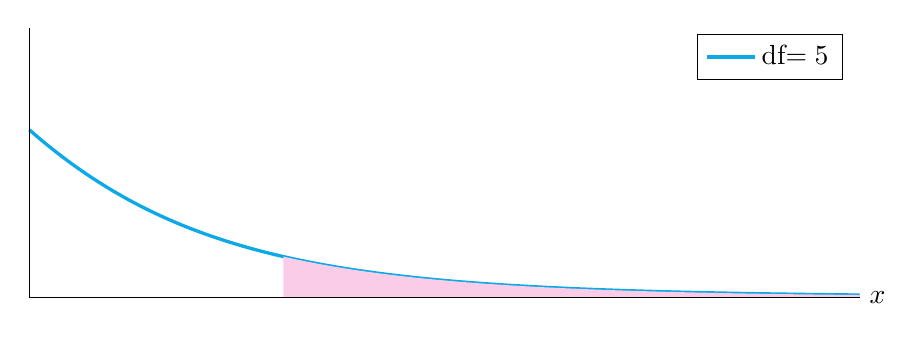
\begin{tikzpicture}[declare function={gamma(\z)=
    2.506628274631*sqrt(1/\z)+ 0.20888568*(1/\z)^(1.5)+ 0.00870357*(1/\z)^(2.5)- (174.2106599*(1/\z)^(3.5))/25920- (715.6423511*(1/\z)^(4.5))/1244160)*exp((-ln(1/\z)-1)*\z;},%
    declare function={student(\x,\n)= gamma((\n+1)/2.)/(sqrt(\n*pi) *gamma(\n/2.)) *((1+(\x*\x)/\n)^(-(\n+1)/2.));}%
    ]%
        \begin{axis}[
        no markers, %
        ymax=0.2, %
        ymin=0, %
        domain=1.5:5, %
        samples=100, %
        axis lines*=left, %
        xlabel=$x$, %
        every axis y label/.style={at=(current axis.above origin),anchor=south}, %
        every axis x label/.style={at=(current axis.right of origin),anchor=west}, %
        height=5cm, %
        width=\linewidth, %
        xtick=\empty, %
        xticklabels=\empty, %
        ytick=\empty, %
        enlargelimits=false, %
        clip=false, %
        axis on top, %
        grid = major, %
        legend entries={df$=5$}]
        \addplot [very thick,smooth, cyan!95!black, domain=1.5:5] {student(x,5)};%
        \addplot [very thick,smooth, cyan!95!black,fill=magenta!20, draw=none, domain=2.571:5] {student(x,5)} \closedcycle;%
    \end{axis}%
    \end{tikzpicture}%
    \caption{}%
    \label{fig:tdist1a}%
\end{subfigure}%
\hfill %
\begin{subfigure}[b]{0.31\linewidth}%
    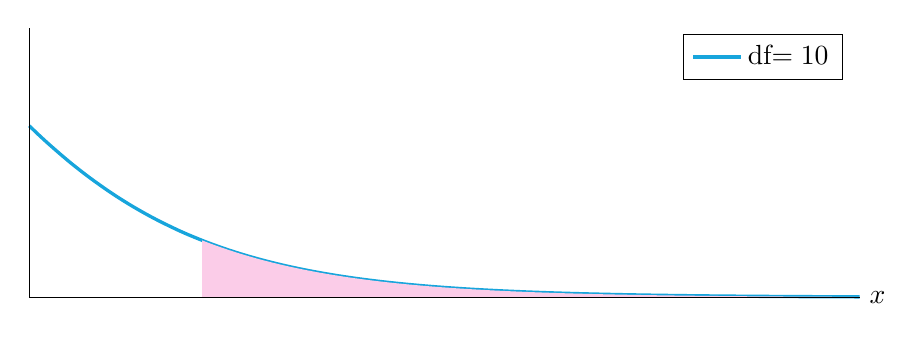
\begin{tikzpicture}[declare function={gamma(\z)=
    2.506628274631*sqrt(1/\z)+ 0.20888568*(1/\z)^(1.5)+ 0.00870357*(1/\z)^(2.5)- (174.2106599*(1/\z)^(3.5))/25920- (715.6423511*(1/\z)^(4.5))/1244160)*exp((-ln(1/\z)-1)*\z;},%
    declare function={student(\x,\n)= gamma((\n+1)/2.)/(sqrt(\n*pi) *gamma(\n/2.)) *((1+(\x*\x)/\n)^(-(\n+1)/2.));}%
    ]%
        \begin{axis}[
        no markers, %
        ymin=0, %
        ymax=0.2, %
        domain=1.5:5, %
        samples=100, %
        axis lines*=left, %
        xlabel=$x$, %
        every axis y label/.style={at=(current axis.above origin),anchor=south}, %
        every axis x label/.style={at=(current axis.right of origin),anchor=west}, %
        height=5cm, %
        width=\linewidth, %
        xtick=\empty, %
        xticklabels=\empty, %
        ytick=\empty, %
        enlargelimits=false, %
        clip=false, %
        axis on top, %
        grid = major, %
        legend entries={df$=10$}]
        \addplot [very thick,smooth, cyan!90!black, domain=1.5:5] {student(x,10)};%
        \addplot [very thick,smooth, cyan!90!black, fill=magenta!20, draw=none, domain=2.228:5] {student(x,10)} \closedcycle;%
    \end{axis}%
    \end{tikzpicture}%
    \caption{}%
    \label{fig:tdist1b}%
\end{subfigure}%
\hfill %
\begin{subfigure}[b]{0.31\linewidth}%
    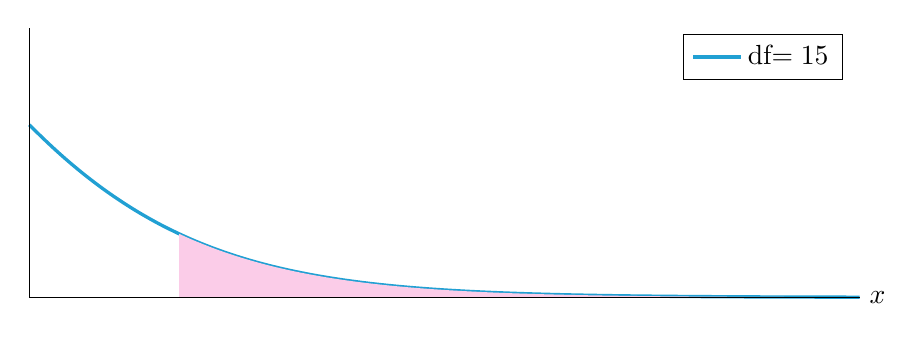
\begin{tikzpicture}[declare function={gamma(\z)=
    2.506628274631*sqrt(1/\z)+ 0.20888568*(1/\z)^(1.5)+ 0.00870357*(1/\z)^(2.5)- (174.2106599*(1/\z)^(3.5))/25920- (715.6423511*(1/\z)^(4.5))/1244160)*exp((-ln(1/\z)-1)*\z;},%
    declare function={student(\x,\n)= gamma((\n+1)/2.)/(sqrt(\n*pi) *gamma(\n/2.)) *((1+(\x*\x)/\n)^(-(\n+1)/2.));}%
    ]%
        \begin{axis}[
        no markers, %
        ymax=0.2, %
        ymin=0, %
        domain=1.5:5, %
        samples=100, %
        axis lines*=left, %
        xlabel=$x$, %
        every axis y label/.style={at=(current axis.above origin),anchor=south}, %
        every axis x label/.style={at=(current axis.right of origin),anchor=west}, %
        height=5cm, %
        width=\linewidth, %
        xtick=\empty, %
        xticklabels=\empty, %
        ytick=\empty, %
        enlargelimits=false, %
        clip=false, %
        axis on top, %
        grid = major, %
        legend entries={df$=15$}]
        \addplot [very thick,smooth, cyan!85!black, domain=1.5:5] {student(x,15)};%
        \addplot [very thick,smooth, cyan!85!black, fill=magenta!20, draw=none, domain=2.131:5] {student(x,15)} \closedcycle;%
    \end{axis}%
    \end{tikzpicture}%
    \caption{}%
    \label{fig:tdist1c}%
\end{subfigure}%
\\[1ex]
\begin{subfigure}[b]{0.31\linewidth}%
    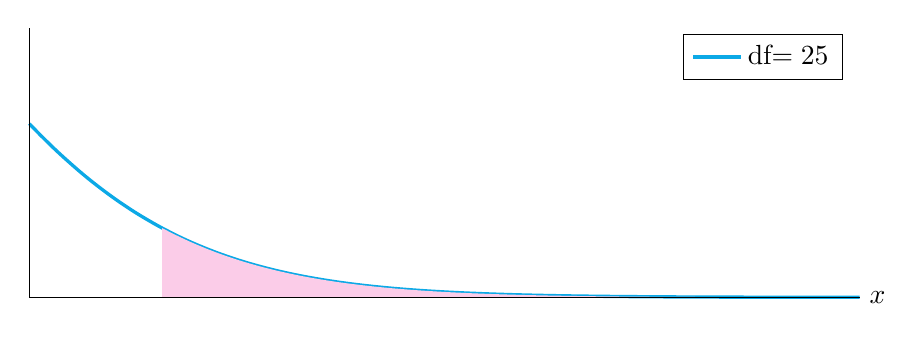
\begin{tikzpicture}[declare function={gamma(\z)=
    2.506628274631*sqrt(1/\z)+ 0.20888568*(1/\z)^(1.5)+ 0.00870357*(1/\z)^(2.5)- (174.2106599*(1/\z)^(3.5))/25920- (715.6423511*(1/\z)^(4.5))/1244160)*exp((-ln(1/\z)-1)*\z;},%
    declare function={student(\x,\n)= gamma((\n+1)/2.)/(sqrt(\n*pi) *gamma(\n/2.)) *((1+(\x*\x)/\n)^(-(\n+1)/2.));}%
    ]%
        \begin{axis}[
        no markers, %
        ymax=0.2, %
        ymin=0, %
        domain=1.5:5, %
        samples=100, %
        axis lines*=left, %
        xlabel=$x$, %
        every axis y label/.style={at=(current axis.above origin),anchor=south}, %
        every axis x label/.style={at=(current axis.right of origin),anchor=west}, %
        height=5cm, %
        width=\linewidth, %
        xtick=\empty, %
        xticklabels=\empty, %
        ytick=\empty, %
        enlargelimits=false, %
        clip=false, %
        axis on top, %
        grid = major, %
        legend entries={df$=25$}]
        \addplot [very thick,smooth, cyan!95!black, domain=1.5:5] {student(x,25)};%
        \addplot [very thick,smooth, cyan!95!black,fill=magenta!20, draw=none, domain=2.060:5] {student(x,25)} \closedcycle;%
    \end{axis}%
    \end{tikzpicture}%
    \caption{}%
    \label{fig:tdist1d}%
\end{subfigure}%
\hfill %
\begin{subfigure}[b]{0.31\linewidth}%
    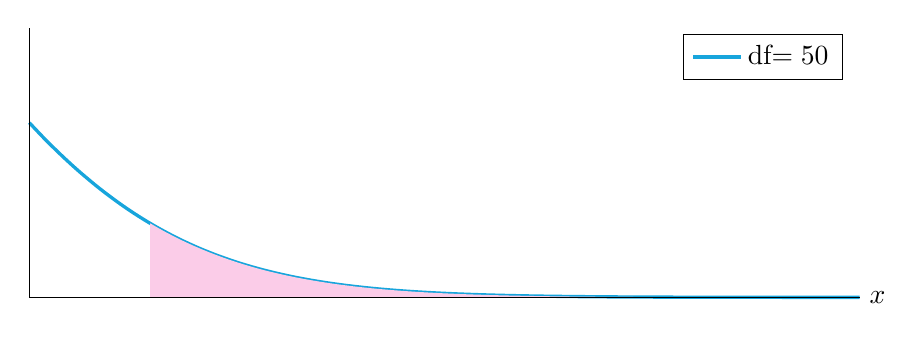
\begin{tikzpicture}[declare function={gamma(\z)=
    2.506628274631*sqrt(1/\z)+ 0.20888568*(1/\z)^(1.5)+ 0.00870357*(1/\z)^(2.5)- (174.2106599*(1/\z)^(3.5))/25920- (715.6423511*(1/\z)^(4.5))/1244160)*exp((-ln(1/\z)-1)*\z;},%
    declare function={student(\x,\n)= gamma((\n+1)/2.)/(sqrt(\n*pi) *gamma(\n/2.)) *((1+(\x*\x)/\n)^(-(\n+1)/2.));}%
    ]%
        \begin{axis}[
        no markers, %
        ymax=0.2, %
        ymin=0, %
        domain=1.5:5, %
        samples=100, %
        axis lines*=left, %
        xlabel=$x$, %
        every axis y label/.style={at=(current axis.above origin),anchor=south}, %
        every axis x label/.style={at=(current axis.right of origin),anchor=west}, %
        height=5cm, %
        width=\linewidth, %
        xtick=\empty, %
        xticklabels=\empty, %
        ytick=\empty, %
        enlargelimits=false, %
        clip=false, %
        axis on top, %
        grid = major, %
        legend entries={df$=50$}]
        \addplot [very thick,smooth, cyan!90!black, domain=1.5:5] {student(x,50)};%
        \addplot [very thick,smooth, cyan!90!black, fill=magenta!20, draw=none, domain=2.009:5] {student(x,50)} \closedcycle;%
    \end{axis}%
    \end{tikzpicture}%
    \caption{}%
    \label{fig:tdist1e}%
\end{subfigure}%
\hfill %
\begin{subfigure}[b]{0.31\linewidth}%
    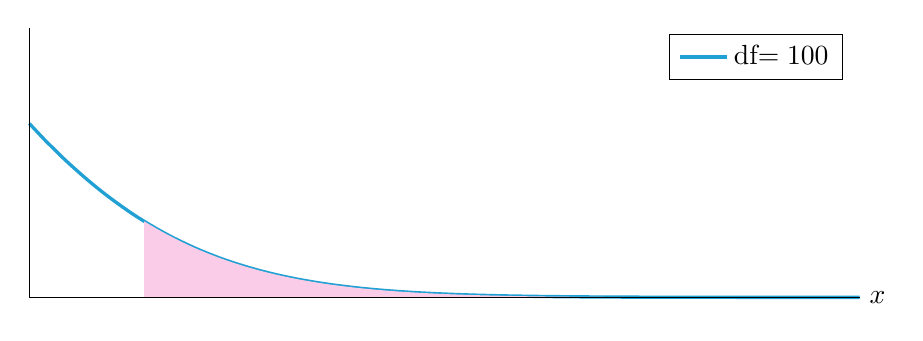
\begin{tikzpicture}[declare function={gamma(\z)=
    2.506628274631*sqrt(1/\z)+ 0.20888568*(1/\z)^(1.5)+ 0.00870357*(1/\z)^(2.5)- (174.2106599*(1/\z)^(3.5))/25920- (715.6423511*(1/\z)^(4.5))/1244160)*exp((-ln(1/\z)-1)*\z;},%
    declare function={student(\x,\n)= gamma((\n+1)/2.)/(sqrt(\n*pi) *gamma(\n/2.)) *((1+(\x*\x)/\n)^(-(\n+1)/2.));}%
    ]%
        \begin{axis}[
        no markers, %
        ymax=0.2, %
        ymin=0, %
        domain=1.5:5, %
        samples=100, %
        axis lines*=left, %
        xlabel=$x$, %
        every axis y label/.style={at=(current axis.above origin),anchor=south}, %
        every axis x label/.style={at=(current axis.right of origin),anchor=west}, %
        height=5cm, %
        width=\linewidth, %
        xtick=\empty, %
        xticklabels=\empty, %
        ytick=\empty, %
        enlargelimits=false, %
        clip=false, %
        axis on top, %
        grid = major, %
        legend entries={df$=100$}]
        \addplot [very thick,smooth, cyan!85!black, domain=1.5:5] {student(x,100)};%
        \addplot [very thick,smooth, cyan!85!black, fill=magenta!20, draw=none, domain=1.984:5] {student(x,100)} \closedcycle;%
    \end{axis}%
    \end{tikzpicture}%
    \caption{}%
    \label{fig:tdist1f}%
\end{subfigure}%
\caption{As the degrees of freedom increases, you can see that the shaded red area moves to the left so it appears that the shaded area is increasing. In actuality, the shaded red area is the same (representing $2.5\%$) and it appears to be changing due to changing graph shape. For small degrees of freedom, the shape of the bell curve is flat with long fat tails, and as df increases the bell curve reforms to look like that of the standard normal distribution.}%
\label{fig:tdist1}%
\end{figure}%
\FloatBarrier

\clearpage
\phantomsection
\subsection*{Math expressions}
\addcontentsline{toc}{subsection}{Math expressions}
Reading equations and understanding mathematical operations can be a little confusing, especially when you're not so sure about the consequences of making an incorrect inference. Firstly, fractions: what to do when you have a fraction on the denominator? When you divide by a whole number you can easily imagine this as sharing a cake with friends, e.g. divide by 5 can be pictured as taking the numerator (the cake) and cutting it into 5 pieces. When you divide by a fraction, you can't really imagine it so well as it doesn't make sense in terms of the cake analogy. If you convert the fraction in the denominator into a decimal number it can be a little more easy to understand: take the following fraction
\begin{align}
    \frac{1}{\sfrac{1}{2}} &= \frac{1}{0.5}
    \intertext{If you take a whole cake and divide it by a half, you are actually dividing it by $0.5$. What you are asking is, ``how many $0.5$'s can you fit into 1'' or ``how many half cakes make up a whole cake''? With this thought in mind, we can easily conclude that 2 halves make a whole, so the answer is 2. The easiest way to do this is by the 'ole flip and multiply:}
    \frac{1}{\sfrac{1}{2}} &= \frac{1}{1} \times \frac{2}{1} = 2.
\end{align}
This method is better than thinking always in cakes, as you may not always have a nice fraction with integers to work with. Consider the following fraction:
\begin{align}
    \frac{8}{\sfrac{5}{6}} &= \frac{8}{0.8\bar{3}}
    \intertext{In terms of cakes, you are asking ``how many $0.8\bar{3}$'s of a cake fit into 8 cakes''? You can easily think that there are at least 8 $0.8\bar{3}$'s of a cake in 8 cakes as $0.8\bar{3}$ is less than 1. So, now you have left over $0.1\bar{6}$ from each of the 8 cakes, which equates to $8 \times (1/6) = 8/6$. We can write this fraction as $(3+5)/6 =(3/6) + (5/6) = 0.5 + 0.8\bar{3}$, meaning that we can in total fit 9 $0.8\bar{3}$'s of a cake in 8 cakes and we will have half of a cake left over. Now comes the tricky part, what proportion of $0.8\bar{3}$ of a cake makes up half a cake. This is why we only visualise fractions in terms of cakes when the fractions are ``nice''. The easier way is to flip and multiply:}
    \frac{8}{\sfrac{5}{6}} &= \frac{8}{1} \times \frac{6}{5} = \frac{48}{5} = 9 + \frac{3}{5} = 9.6.
    \intertext{What are you actually doing here? You don't want the fraction in the denominator, so you \textbf{multiply it out}:}
    \frac{8}{\sfrac{5}{6}} = x \implies 
    \brac{\sfrac{5}{6}} \times \brac{\frac{8}{\sfrac{5}{6}}} &= \brac{\sfrac{5}{6}} \times \brac{x} 
    \intertext{We don't know what $\frac{8}{\sfrac{5}{6}}$ is yet, so we set it equal to unknown $x$. The next step (seen above) is to multiply both sides by the denominator $\sfrac{5}{6}$, which then requires that we solve for $x$ and you will see that we get the same answer.}
    \implies 8 &= \frac{5x}{6} \\
    \implies 8 \times 6 = 48 &= 5x \\
    \implies \frac{48}{5} = 9.6 &= x.
\end{align}
It doesn't really matter which of the three methods you choose to use: cakes, flip-a-roo, or multiplying it out. The important thing to remember is make it easiest for you; I would recommend the multiplying out method as it will make sure you don't make any errors. Thus far we have dealt with fractions in an arbitrary sense, however let's apply it to something which is more relevant. In the previous sections, we saw that we can calculate power if we know $\mu_A$ and you have heard that you can use effect size to calculate power. 
\begin{align}
    \text{power} &= 
    \begin{dcases}
    \given{\frac{\bar{X} - \mu_0}{\sigma /\sqrt{n}}> z_{1 - \alpha/2}}{\mu=\mu_A} , & H_A: \; \mu\ne\mu_0 \text{ and } \mu_A>\mu_0; \\
    \given{\frac{\bar{X} - \mu_0}{\sigma /\sqrt{n}}< -z_{1 - \alpha/2}}{\mu=\mu_A} , & H_A: \; \mu\ne\mu_0 \text{ and } \mu_0>\mu_A; \\
    \given{\frac{\bar{X} - \mu_0}{\sigma /\sqrt{n}}> z_{1 - \alpha}}{\mu=\mu_A}, & H_A: \; \mu>\mu_0; \\
    \given{\frac{\bar{X} - \mu_0}{\sigma /\sqrt{n}}< -z_{1 - \alpha}}{\mu=\mu_A}, & H_A: \; \mu>\mu_0.
    \end{dcases} \\
    &= 
    \begin{dcases}
    \pr{Z> \frac{\mu_0 - \mu_A}{\sigma /\sqrt{n}} + z_{1 - \alpha/2}} , & H_A: \; \mu\ne\mu_0 \text{ and } \mu_A>\mu_0; \\
    \pr{Z< \frac{\mu_0 - \mu_A}{\sigma /\sqrt{n}} -z_{1 - \alpha/2}} , & H_A: \; \mu\ne\mu_0 \text{ and } \mu_0>\mu_A; \\
    \pr{Z> \frac{\mu_0 - \mu_A}{\sigma /\sqrt{n}} + z_{1 - \alpha}}, & H_A: \; \mu>\mu_0; \\
    \pr{Z< \frac{\mu_0 - \mu_A}{\sigma /\sqrt{n}} -z_{1 - \alpha}}, & H_A: \; \mu>\mu_0.
    \end{dcases} 
    \intertext{The above four cases are the usual ones that you will come across in this course, as you are mostly concerned about means. Suppose you want a specific power for your test, so you are looking for a particular critical $z$-value corresponding to}
    &= 1 - \beta = \pr{Z<z_{1-\beta}} 
\end{align}
For instance, if you require 80\% power, then $z_{1 - \beta} = 0.85$ and so you need to solve $0.85> \frac{\mu_0 - \mu_A}{\sigma /\sqrt{n}} + z_{1 - \alpha/2}$, for $H_A:$ $\mu\ne\mu_0$ and $\mu_A>\mu_0$. You need to solve the following equations for $n$:
\begin{align}
    z_{1 - \beta} &> \frac{\mu_0 - \mu_A}{\sigma /\sqrt{n}} + z_{1 - \alpha/2} , & H_A: \; \mu\ne\mu_0 \text{ and } \mu_A>\mu_0; \\
    z_{1 - \beta} &< \frac{\mu_0 - \mu_A}{\sigma /\sqrt{n}} -z_{1 - \alpha/2} , & H_A: \; \mu\ne\mu_0 \text{ and } \mu_0>\mu_A; \\
    z_{1 - \beta} &> \frac{\mu_0 - \mu_A}{\sigma /\sqrt{n}} + z_{1 - \alpha}, & H_A: \; \mu>\mu_0; \\
    z_{1 - \beta} &< \frac{\mu_0 - \mu_A}{\sigma /\sqrt{n}} -z_{1 - \alpha}, & H_A: \; \mu>\mu_0.
    \intertext{We go about solving these equations in the following way: first subtract the $z(\alpha)$ critical values from both sides.}
    \brac{z_{1 - \beta}} - \brac{z_{1 - \alpha/2}} &> \brac{\frac{\mu_0 - \mu_A}{\sigma /\sqrt{n}} + z_{1 - \alpha/2}} - \brac{z_{1 - \alpha/2}} , & H_A: \; \mu\ne\mu_0 \text{ and } \mu_A>\mu_0; \\
    \brac{z_{1 - \beta}} - \brac{-z_{1 - \alpha/2}} &< \brac{\frac{\mu_0 - \mu_A}{\sigma /\sqrt{n}} -z_{1 - \alpha/2}} - \brac{-z_{1 - \alpha/2}} , & H_A: \; \mu\ne\mu_0 \text{ and } \mu_0>\mu_A; \\
    \brac{z_{1 - \beta}} - \brac{z_{1 - \alpha}} &> \brac{\frac{\mu_0 - \mu_A}{\sigma /\sqrt{n}} + z_{1 - \alpha}} - \brac{z_{1 - \alpha}}, & H_A: \; \mu>\mu_0; \\
    \brac{z_{1 - \beta}} - \brac{-z_{1 - \alpha}} &< \brac{\frac{\mu_0 - \mu_A}{\sigma /\sqrt{n}} -z_{1 - \alpha}} - \brac{-z_{1 - \alpha}}, & H_A: \; \mu>\mu_0.
    \intertext{Next, we multiply out the fraction in the denominator.}
    \brac{\frac{\sigma}{\sqrt{n}}} \times \brac{z_{1 - \beta} - z_{1 - \alpha/2}} &> \brac{\frac{\sigma}{\sqrt{n}}} \times \brac{\frac{\mu_0 - \mu_A}{\sigma /\sqrt{n}}} , & H_A: \; \mu\ne\mu_0 \text{ and } \mu_A>\mu_0; \\
    \brac{\frac{\sigma}{\sqrt{n}}} \times \brac{z_{1 - \beta} + z_{1 - \alpha/2}} &< \brac{\frac{\sigma}{\sqrt{n}}} \times \brac{\frac{\mu_0 - \mu_A}{\sigma /\sqrt{n}}}, & H_A: \; \mu\ne\mu_0 \text{ and } \mu_0>\mu_A; \\
    \brac{\frac{\sigma}{\sqrt{n}}} \times \brac{z_{1 - \beta} - z_{1 - \alpha}} &> \brac{\frac{\sigma}{\sqrt{n}}} \times \brac{\frac{\mu_0 - \mu_A}{\sigma /\sqrt{n}}}, & H_A: \; \mu>\mu_0; \\
    \brac{\frac{\sigma}{\sqrt{n}}} \times \brac{z_{1 - \beta} + z_{1 - \alpha}} &< \brac{\frac{\sigma}{\sqrt{n}}} \times \brac{\frac{\mu_0 - \mu_A}{\sigma /\sqrt{n}}}, & H_A: \; \mu>\mu_0.
    \intertext{Now we multiply both sides by $\sqrt{n}$}
    \brac{\sqrt{n}} \times \brac{\frac{\sigma \brac{z_{1 - \beta} - z_{1 - \alpha/2}}}{\sqrt{n}}} &> \brac{\sqrt{n}} \times \brac{\mu_0 - \mu_A}, & H_A: \; \mu\ne\mu_0 \text{ and } \mu_A>\mu_0; \\
    \brac{\sqrt{n}} \times \brac{\frac{\sigma \brac{z_{1 - \beta} + z_{1 - \alpha/2}}}{\sqrt{n}}} &< \brac{\sqrt{n}} \times \brac{\mu_0 - \mu_A}, & H_A: \; \mu\ne\mu_0 \text{ and } \mu_0>\mu_A; \\
    \brac{\sqrt{n}} \times \brac{\frac{\sigma \brac{z_{1 - \beta} - z_{1 - \alpha}}}{\sqrt{n}}} &> \brac{\sqrt{n}} \times \brac{\mu_0 - \mu_A}, & H_A: \; \mu>\mu_0; \\
    \brac{\sqrt{n}} \times \brac{\frac{\sigma \brac{z_{1 - \beta} + z_{1 - \alpha}}}{\sqrt{n}}} &< \brac{\sqrt{n}} \times \brac{\mu_0 - \mu_A}, & H_A: \; \mu>\mu_0.
    \intertext{Finally, we divide by $\mu_0 - \mu_A$:}
    \brac{\frac{1}{\mu_0 - \mu_A}} \times \brac{\sigma \brac{z_{1 - \beta} - z_{1 - \alpha/2}}} &> \brac{\frac{1}{\mu_0 - \mu_A}} \times \brac{\sqrt{n}\brac{\mu_0 - \mu_A}}, & H_A: \; \mu\ne\mu_0 \text{ and } \mu_A>\mu_0; \\
    \brac{\frac{1}{\mu_0 - \mu_A}} \times \brac{\sigma \brac{z_{1 - \beta} + z_{1 - \alpha/2}}} &< \brac{\frac{1}{\mu_0 - \mu_A}} \times \brac{\sqrt{n}\brac{\mu_0 - \mu_A}}, & H_A: \; \mu\ne\mu_0 \text{ and } \mu_0>\mu_A; \\
    \brac{\frac{1}{\mu_0 - \mu_A}} \times \brac{\sigma \brac{z_{1 - \beta} - z_{1 - \alpha}}} &> \brac{\frac{1}{\mu_0 - \mu_A}} \times \brac{\sqrt{n}\brac{\mu_0 - \mu_A}}, & H_A: \; \mu>\mu_0; \\
    \brac{\frac{1}{\mu_0 - \mu_A}} \times \brac{\sigma \brac{z_{1 - \beta} + z_{1 - \alpha}}} &< \brac{\frac{1}{\mu_0 - \mu_A}} \times \brac{\sqrt{n}\brac{\mu_0 - \mu_A}}, & H_A: \; \mu>\mu_0.
    \intertext{Recalling the general formula for Cohen's $d = (\mu_1 - \mu_2)/\sigma$}
\end{align}

